\problemname{Flappy Bird}

Help the bird Faby to navigate through a sequence of $n$ pairs of pipes, by finding the shortest line he can fly on to reach his destination. For simplicity, we represent Faby as a single point in the plane and assume every pipe has width zero. This way, the gap between every pair of pipes can be represented as an interval on the $y$ axis. The bird starts out at $s = (x_s, y_s)$ and his goal is to reach $t = (x_t, y_t)$. Find the shortest line from $s$ to $t$, passing through all intervals in between in increasing order of their $x$ coordinates.

\begin{figure}[!h]
  \centering
  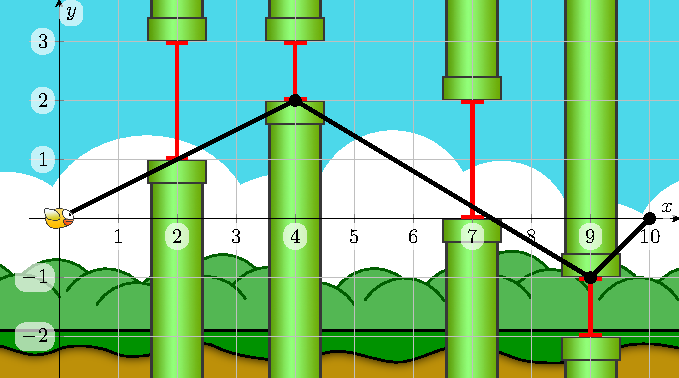
\includegraphics[width=0.7\textwidth]{sample2}
  \caption{Visualisation of the second sample input. The red lines represent the intervals and the black line the shortest possible path. Faby and the black dots are the points in the output. Note that $(2, 1)$ can optionally be included in the output too.}
\end{figure}

\section*{Input}
The input consists of:
\begin{itemize}
	\item One line with four integers $x_s, y_s, x_t$ and $y_t$ ($-10^9 \le x_s, y_s, x_t, y_t \le 10^9$), the start and end points.
	\item One line with an integer $n\ (0 \le n \le 10^6)$, the number of intervals.
	\item $n$ lines, the $i$th of which contains three integer $x_i, y_{i,1}$ and $y_{i,2}$ ($-10^9 \le x_i, y_{i, 1}, y_{i, 2} \le 10^9$, $y_{i, 1} < y_{i, 2}$), the intervals.
\end{itemize}
It can be assumed that $x_s < x_1 < \dots < x_n < x_t$.

\section*{Output}
Output a sequence of $k$ $(2 \le k \le n+2$) points $p_1, \dots, p_k$, one per line, such that:
\begin{itemize}
	\item All points have integer coordinates.
	\item $p_1 = s$ and $p_k = t$.
	\item Let $P$ be the path obtained by connecting $\overline{p_i p_{i+1}}$ for all $1 \le i < k$. Then:
	\begin{itemize}
		\item $P$ passes through all intervals in increasing order of their $x$ coordinates.
		\item The length of $P$ is minimal.
	\end{itemize}
\end{itemize}
If there are multiple valid solutions, you may output any one of them.
